\documentclass[12pt, a4paper, onecolumn, oneside, final]{report}

% Load konfigurasi LaTeX untuk tipe laporan thesis
\usepackage{src/unpam}
\usepackage{enumitem}
\usepackage{array}
\usepackage{graphics}
\usepackage{microtype}
\usepackage{adjustbox}
\usepackage[numbers]{natbib}



% %%%%%%%%%%%%%%%%%%%%%%%%%%%%%%%%%%%%%%%%%%%%%%%%%%%%%%%%%%
% %%%%%%%%%%%%%%%%%%%%%%%%%%%%%%%%%%%%%%%%%%%%%%%%%%%%%%%%%%
% Variabel baru untuk menyimpan nomor halaman
\newcounter{originalpagenumber}

% Awal bagian penulisan laporan
\begin{document}

%
% Hyphenation untuk Indonesia 
%
% @author  Enggar Alfianto
% @version 1.00
% 
% Tambahkan cara pemenggalan kata-kata yang salah dipenggal secara otomatis 
% oleh LaTeX. Jika kata tersebut dapat dipenggal dengan benar, maka tidak 
% perlu ditambahkan dalam berkas ini. Tanda pemenggalan kata menggunakan 
% tanda '-'; contoh:
% menarik
%   --> pemenggalan: me-na-rik
%

\hyphenation{
    % alphabhet A
    a-na-li-sa a-tur
    a-pli-ka-si
    a-na-li-tik
    % alphabhet B
    ba-ngun-an
    be-be-ra-pa
    ber-ge-rak
    ber-ke-lan-jut-an
    ber-pe-nga-ruh
    bim-bing-an
    % alphabhet C
    ca-ri
    % alphabhet D
    di-sim-pan di-pim-pin de-ngan da-e-rah di-ba-ngun da-pat di-nya-ta-kan
    di-sim-bol-kan di-pi-lih di-li-hat de-fi-ni-si
    di-rahmat-i
    di-identifi-kasi-kan
    di-re-pre-sen-ta-si-kan
    du-kung-an-nya
    % alphabhet E
    e-ner-gi eks-klu-sif
    % alphabhet F
    fa-si-li-tas
    fe-no-me-na
    % alphabhet G
    ga-bung-an ge-rak
    % alphabhet H
    ha-lang-an
    hamilton-nia-nya
    % alphabhet I
    % alphabhet J
    % alphabhet K
    ke-rapat-an
    ke-hi-lang-an
    ku-ning
    kompu-tasi
    kua-li-tas ka-me-ra ke-mung-kin-an ke-se-pa-ham-an
    % alphabhet L
    ling-kung-an
    % alphabhet M
    me-nge-luar-kan
    me-neng-ah
    mem-perhitung-kan
    mem-ban-ding-kan
    meng-a-tas-i me-mung-kin-kan me-nge-na-i me-ngi-rim-kan
    meng-u-bah meng-a-dap-ta-si me-nya-ta-kan mo-di-fi-ka-si
    meng-a-tur
    micro-service
    % alphabhet N
    nya-ta non-eks-klu-sif
    nano-tekno-logi
    % alphabhet O
    % alphabhet P
    pa-ling
    pe-nye-rap-an
    pe-ngon-trol
    pe-mo-del-an
    pe-ran  pe-ran-an-nya
    pem-ba-ngun-an pre-si-den pe-me-rin-tah prio-ri-tas peng-am-bil-an
    peng-ga-bung-an pe-nga-was-an pe-ngem-bang-an
    pe-nga-ruh pa-ra-lel-is-me per-hi-tung-an per-ma-sa-lah-an
    pen-ca-ri-an peng-struk-tur-an
    % alphabhet Q
    % alphabhet R
    ran-cang-an
    % alphabhet S
    si-mu-la-si sa-ngat
    se-bagai
    semi-konduktor
    % alphabhet T
    te-ngah
    ter-da-pat
    ter-selesai-kanya
    % alphabhet U
    % alphabhet V
    % alphabhet W
    % alphabhet X
    % alphabhet Y
    % alphabhet Z
    % special
}

% Sampul Laporan
\begin{titlepage}
    \begin{center}
        \onehalfspacing
        \large \bfseries \textit{Automatic Deployment}  Aplikasi berbasis \textit{Microservice} Pada Platform Kubernetes Dengan Metode \textit{Pull-Up} \\
        \vspace{1cm}
        \large Laporan Tugas Akhir \\
        \vspace{0.5cm}

        {\small \normalfont Diajukan Untuk Memenuhi\\
            Persyaratan Guna Meraih Gelar Sarjana\\
            Informatika Universitas Muhammadiyah Malang}
        \vspace{2cm}

        
\includegraphics[width=6cm]{figures/logo_umm.png}

        \vspace{1cm}
        \normalfont \normalsize Muhammad Zein Ihza Fahrozi \\
        \normalfont \normalsize 201810370311072 \\

        \vspace{1cm}
        \bfseries \normalsize Bidang Minat \\
        \normalfont \normalsize Rekayasa Perangkat Lunak

        \vspace{2.5cm}

        \normalsize PROGRAM STUDI TEKNIK INFORMATIKA FAKULTAS TEKNIK \\
        UNIVERSITAS MUHAMMADIYAH MALANG \\
        2021



    \end{center}

\end{titlepage}

\newpage

% Daftar isi, gambar, dan tabel
% Gunakan penomeran Romawi (i, ii, iii, ...) setelah bagian ini.
\pagenumbering{roman}

% Lembar Persetujuan
\phantomsection \addcontentsline{toc}{chapter}{LEMBAR PERSETEJUAN}
\chapter*{\uppercase{LEMBAR PERSETUJUAN}}
\vspace{1cm}

\begin{center}
    ``To Be Added Bismillah''
\end{center}

\newpage

% Lembar Pengesahan
\phantomsection \addcontentsline{toc}{chapter}{LEMBAR PENGESAHAN}
\chapter*{\uppercase{LEMBAR PENGESAHAN}}
\vspace{1cm}

\center ``To Be Added Bismillaah''

\newpage

% Lembar Pernyataan
\phantomsection \addcontentsline{toc}{chapter}{LEMBAR PERNYATAAN}
\chapter*{\uppercase{LEMBAR PERNYATAAN}}

\begin{center}
    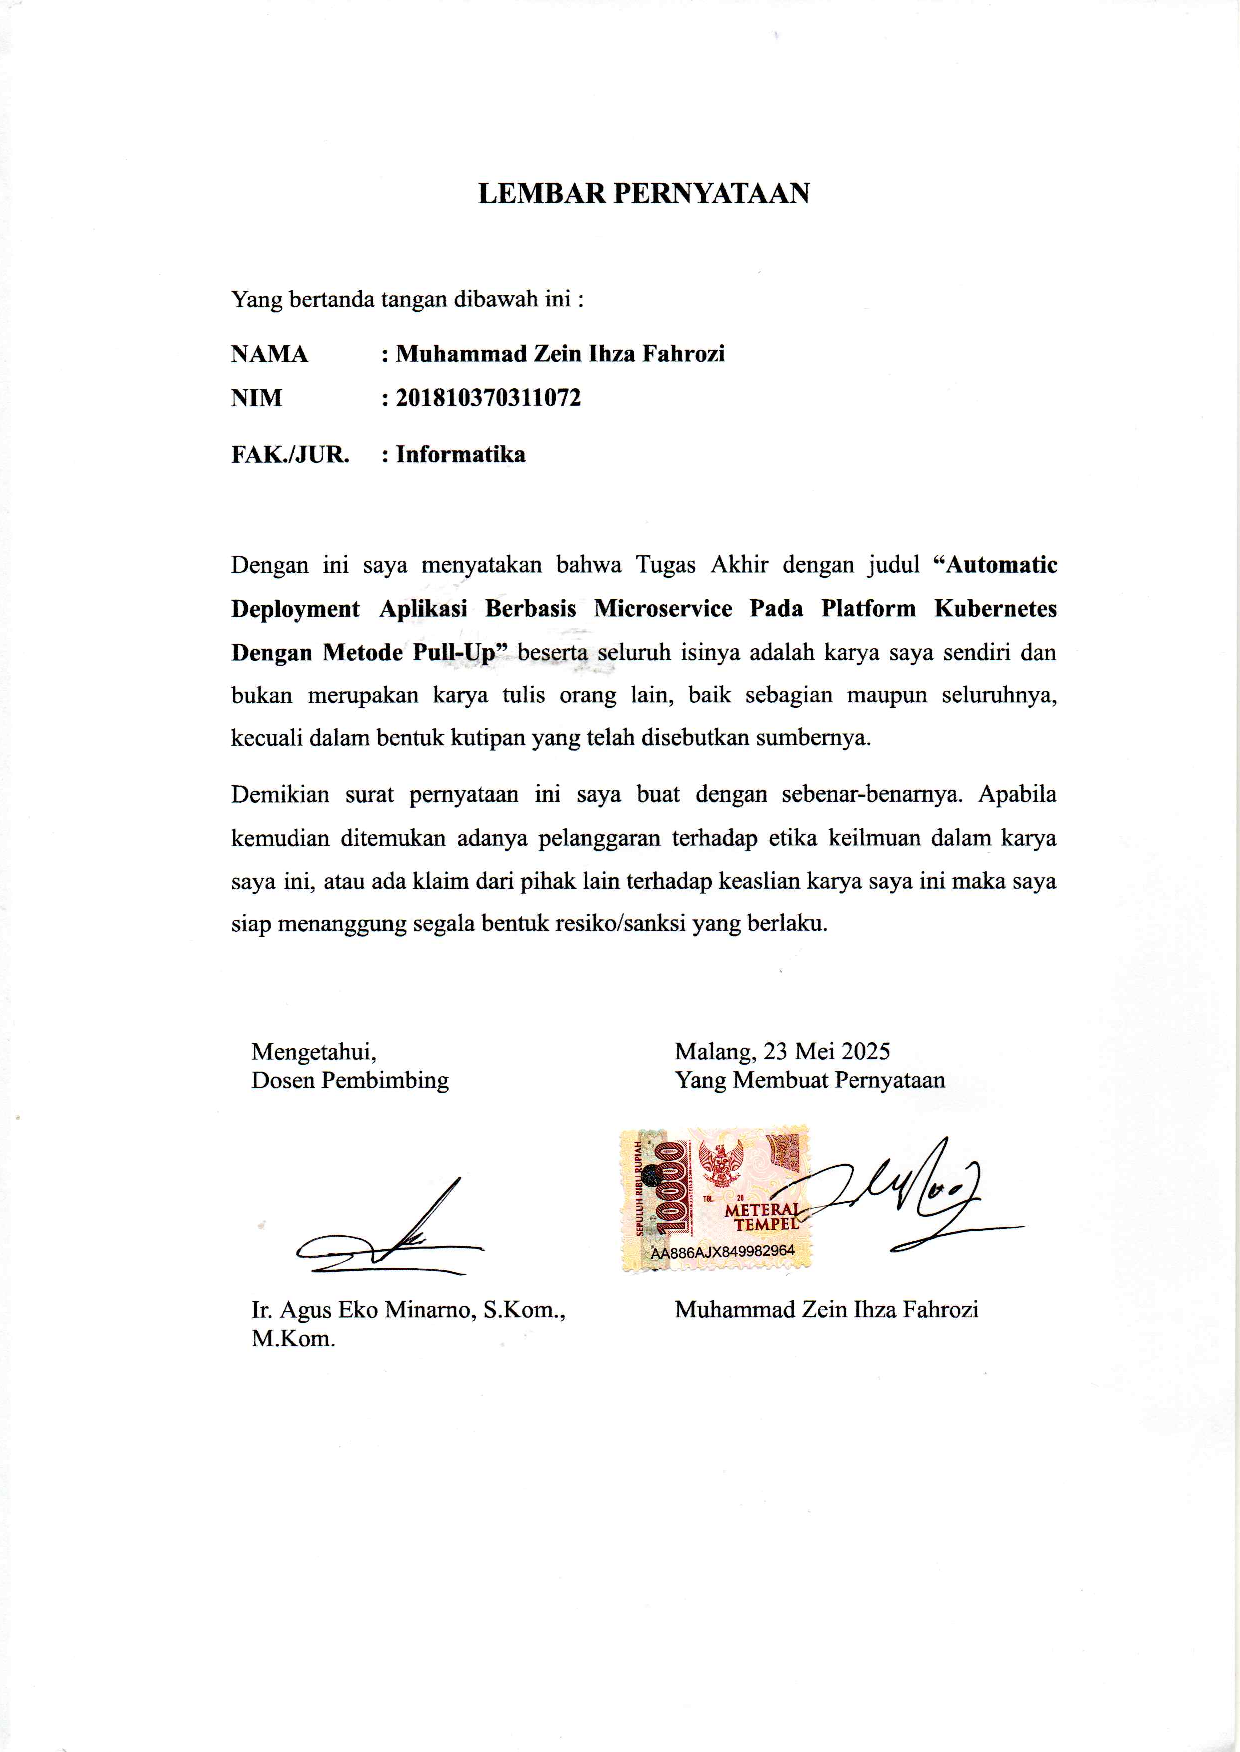
\includegraphics[width=\textwidth,page=1]{misc/lembar-pernyataan-scan.pdf}
\end{center}

\newpage


% Abstrak
%
% Halaman Abstract
\phantomsection \addcontentsline{toc}{chapter}{ABSTRAK}
\chapter*{ABSTRAK}

\begin{singlespace}
	\blindtext \\[20pt]
	Keywords: \textit{Information System, Testing Project}
\end{singlespace}

\newpage

\phantomsection \addcontentsline{toc}{chapter}{ABSTRACT}
\chapter*{ABSTRACT}

\begin{singlespace}
	\blindtext \\[20pt]
	Keywords: \textit{Information System, Testing Project}
\end{singlespace}

\newpage


% Lembar Persembahan
\phantomsection \addcontentsline{toc}{chapter}{LEMBAR PERSEMBAHAN}
\chapter*{\uppercase{LEMBAR PERSEMBAHAN}}
\vspace{1cm}

\begin{center}
    ``To Be Added Bismillah''
\end{center}

\newpage


% Daftar Isi
\vspace*{-2.5cm}
\tableofcontents
\phantomsection \addcontentsline{toc}{chapter}{DAFTAR ISI}
\clearpage
% Daftar Tabel
\vspace*{-2.5cm}
\listoftables
\phantomsection \addcontentsline{toc}{chapter}{DAFTAR TABEL}
\clearpage
% Daftar Gambar
\vspace*{-2.5cm}
\listoffigures
\phantomsection
\addcontentsline{toc}{chapter}{DAFTAR GAMBAR}
\clearpage

% Gunakan penomeran Arab (1, 2, 3, ...) setelah bagian ini.
\pagenumbering{arabic}


%
% Atur header dan footer dalam dokumen.
% 
\renewcommand{\headrulewidth}{0.0pt}
\fancyhf{}
\fancyhead[L]{}
\fancyhead[C]{}
% \fancyhead[R]{\thepage}
\fancyfoot[CO]{\thepage}
\renewcommand{\headrulewidth}{0.0pt}
\renewcommand{\footrulewidth}{0.0pt}
\pagestyle{fancy}

\onehalfspacing
\renewcommand{\chaptername}{BAB}
%-----------------------------------------------------------------------------%
\chapter{PENDAHULUAN}
%-----------------------------------------------------------------------------%
\vspace{4.5pt}
\setlength{\parskip}{0.5em}

\section{Latar Belakang} \label{sec:latar_belakang}
Sebelum digunakan oleh pengguna secara luas, sebuah perangkat lunak perlu
melalui proses \textit{deployment} terlebih dahulu. \textit{Deployment}
perangkat lunak dapat didefinisikan sebagai akuisisi dan eksekusi sebuah
perangkat lunak. Proses ini biasanya dilakukan oleh seorang software deployer
atau yang lebih dikenal saat ini sebagai SRE (site reliability engineer)
\cite{Lyu2007}. Dengan demikian, \textit{deployment} dapat dikatakan sebagai
aktivitas pasca-produksi sebuah perangkat lunak sebelum digunakan oleh
konsumen. Proses \textit{deployment} perangkat lunak terdiri dari beberapa
tahapan yang saling berhubungan, seperti proses rilis perangkat lunak,
instalasi perangkat lunak ke dalam environment eksekusi, dan aktivasi perangkat
lunak \cite{Carzaniga1998}.

Pada saat melakukan \textit{deployment} sebuah sistem perangkat lunak, beberapa
aspek perlu diperhatikan, seperti sub-komponen yang dibutuhkan atau
\textit{package external}, serta \textit{resource} (hardware). Untuk melakukan
\textit{deployment} sub-komponen ini, dibutuhkan sebuah konfigurasi yang
mendeskripsikan versi sub-komponen yang digunakan oleh perangkat lunak. Dengan
bahasa modern sekarang, konfigurasi sub-komponen yang digunakan oleh main
perangkat lunak biasanya sudah dapat dihasilkan secara otomatis, contohnya
adalah; \textit{go modules} \cite{go_mod} dalam bahasa Golang,
\textit{requirement file} \cite{requirementPython} dalam bahasa Python, atau
file \textit{RubySpec} \cite{rubySpec} pada bahasa Ruby.
\par

Terdapat beberapa karakteristik fundamental dalam \textit{deployment} perangkat
lunak yang diidentifikasi oleh Alan Dearle \cite{Dearle2007}, yaitu:

\textbf{\textit{Release}} merupakan tahap penghubung antara proses \textit{deployment} dengan pengembangan perangkat lunak. Tahap ini mencakup seluruh operasi yang diperlukan untuk mempersiapkan sistem sebelum diserahkan kepada pengguna akhir. Aktivitas \textit{release} juga meliputi penentuan sumber daya (\textit{resource}) yang dibutuhkan agar sistem dapat beroperasi dengan optimal pada \textit{environment} yang ditargetkan.

Selanjutnya dilakukan \textit{packaging} terhadap sistem perangkat lunak.
\textit{Package} yang dihasilkan harus memuat seluruh komponen yang dibutuhkan,
termasuk deskripsi sistem, \textit{dependencies} eksternal, prosedur
\textit{deployment}, serta informasi relevan lainnya yang diperlukan untuk
menjalankan sistem pada \textit{environment} tujuan.

\textbf{\textit{Installation}} merupakan tahap persiapan sebelum aktivasi sistem. \textbf{\textit{Activation}} merupakan proses eksekusi perangkat lunak pada waktu tertentu, yang dapat dilakukan melalui antarmuka grafis (\textit{graphical user interface}) atau sebagai layanan latar belakang (\textit{daemon process}).

\textbf{\textit{Updating}} adalah proses penggantian komponen perangkat lunak yang terinstal dengan versi yang lebih baru. Adapun \textbf{\textit{Undeployment}} atau yang dikenal juga sebagai \textit{deinstallation}, merupakan proses penghapusan perangkat lunak yang terinstal dari suatu sistem.
\par
Menurut penelitian yang dilakukan oleh Mockus dkk. \cite{Mockus2005}, kualitas
\textit{deployment} suatu perangkat lunak merupakan salah satu faktor utama
yang mempengaruhi persepsi konsumen terhadap kualitas keseluruhan perangkat
lunak tersebut. Hal senada diungkapkan oleh Jansen dan Brinkkemper
\cite{Jansen2006} yang menyatakan bahwa kelancaran proses \textit{deployment}
merupakan aspek esensial dalam meningkatkan kualitas produk perangkat lunak
suatu perusahaan atau organisasi.

Namun demikian, terdapat beberapa tantangan yang sering dihadapi dalam
pelaksanaan aktivitas \textit{deployment}. Menurut Carzaniga
\cite{Carzaniga1998}, tantangan-tantangan tersebut meliputi:

\begin{itemize}
  \item \textbf{Penggantian Komponen}: Kesulitan dalam melakukan pembaruan (\textit{update}) terhadap komponen sistem yang sedang berjalan tanpa mengganggu layanan.

  \item \textit{\textbf{Dependencies}}: Kompleksitas ketergantungan (\textit{dependencies}) antarkomponen yang harus dikelola dengan hati-hati.

  \item \textbf{Koordinasi}: Perlunya koordinasi yang baik untuk memastikan pembaruan tidak mengganggu proses bisnis yang sedang berjalan.

  \item \textbf{Pluralitas Platform}: Tantangan dalam mengelola \textit{deployment} pada berbagai platform yang berbeda, termasuk kompatibilitas dengan berbagai sistem operasi.
\end{itemize}
\par
Seiring dengan perkembangan teknologi, kompleksitas suatu perangkat lunak
cenderung mengalami peningkatan yang signifikan \cite{Tania2014, Newman2015}.
Pertumbuhan tim pengembang yang diikuti dengan peningkatan kompleksitas
perangkat lunak serta tantangan dalam pemeliharaan (\textit{maintainability})
seringkali menciptakan hambatan (\textit{bottleneck}) dalam siklus
pengembangan. Hal ini pada akhirnya dapat menurunkan efisiensi pengembangan
perangkat lunak secara keseluruhan \cite{Yale2016}.

Untuk mengatasi tantangan ini, diperlukan pendekatan arsitektur yang lebih
baik, salah satunya adalah dengan menerapkan arsitektur \textit{microservice}
\cite{Tania2014}. Konsep \textit{microservice} memungkinkan pengembangan
perangkat lunak dengan memecahnya menjadi komponen-komponen kecil yang terpisah
(\textit{loosely coupled}). Setiap komponen dapat dikembangkan, dijalankan, dan
diatur secara independen oleh tim pengembang yang berbeda \cite{Xiao2017}.

Saat ini, arsitektur \textit{microservice} telah menjadi pilihan utama dalam
pengembangan perangkat lunak yang membutuhkan skalabilitas tinggi
\cite{Wu2014}. Awalnya, implementasi \textit{microservice} dilakukan dengan
memanfaatkan beberapa \textit{Virtual Machine} (VM) yang saling berkomunikasi
melalui protokol REST/HTTP (\textit{Hypertext Transfer Protocol}) atau RPC
(\textit{Remote Procedure Call}) \cite{Khazaei2016}. Namun, pendekatan berbasis
VM ini memiliki beberapa kelemahan, seperti kebutuhan akan operasi manual yang
intensif dan biaya operasional yang relatif tinggi. Hal ini menyebabkan proses
pengembangan dan penskalaan (\textit{scaling}) menjadi lebih kompleks dan
memakan waktu \cite{Khazaei2016}.
\par
Perkembangan teknologi telah menggeser paradigma dari penggunaan
\textit{Virtual Machine} (VM) menuju pendekatan yang lebih modern dalam
merancang arsitektur \textit{microservice}. Teknologi \textit{containerization}
hadir sebagai solusi yang memungkinkan pengemasan perangkat lunak dalam wadah
yang ringkas dan efisien \cite{Khazaei2016}.
\par
Abstraksi yang diberikan oleh \textit{container} tidak hanya menyederhanakan
proses eksekusi, tetapi juga memberikan fleksibilitas yang lebih besar dalam
manajemen sumber daya. Salah satu keunggulan utamanya adalah kemudahan dalam
melakukan penskalaan (\textit{scaling}), di mana penyesuaian kapasitas dapat
dilakukan dengan hanya mengatur jumlah \textit{container} yang berjalan
\cite{Singh2017}.
\par
\textit{Containerization} \cite{davidbritch} membawa dampak signifikan terhadap aspek infrastruktur dan \textit{runtime} dalam pengembangan perangkat lunak. Namun, kehadiran \textit{container} menuntut adanya sistem orkestrasi yang dapat mengelola \textit{container} tersebut secara otomatis.

Kubernetes hadir sebagai solusi dengan menyediakan berbagai fitur canggih,
termasuk \textit{automatic scaling} yang memungkinkan penyesuaian sumber daya
secara dinamis berdasarkan beban kerja \cite{Leila2018, kubernetes_2021}.

Saat ini, proses \textit{deployment} \textit{container} atau \textit{service}
masih sering kali dilakukan secara manual melalui modifikasi konfigurasi
\textit{deployment} berupa file text. Kondisi ini menimbulkan kebutuhan akan
solusi otomatisasi yang dapat menangani proses \textit{deployment} untuk
\textit{service} baru atau yang mengalami perubahan (\textit{update}) secara
lebih efisien.
\par
Dengan banyaknya persaingan dalam dunia perangkat lunak yang terjadi dalam
waktu ini sebuah perusahaan atau pengembang memerlukan waktu yang cepat untuk
melakukan deployment sebuah perangkat lunak. Terdapat beberapa macam workflow
sebuah deploymen perangkat lunak saat ini, tetapi yang industri saat ini
lakukan adalah metode DevOps \cite{Bass2018}. Metode DevOps sendiri merupakan
metode yang digunakan untuk mengembangkan perangkat lunak yang menjembatani
antara dua team yang terisolasi dalam struktur organisasi, contohnya adalah
team pengembang (Dev) dan team operasi (Ops) \cite{Bolscher2019}. Konsep DevOps
\cite{Bass2018} sendiri memungkinkan team pengembang dan operasi untuk
membangun sebuah perangkat lunak yang dapat dijalankan secara otomatis dan
secara berkala dengan menggunakan alat bantu DevOps. Tujuan utama dari itu
adalah untuk meningkatkan kecepatan, reliabilitas, dan perangkat lunak yang
lebih baik. Dalam DevOps sendiri terdapat beberapa sub-metode yang digunakan
yaitu, \textit{Continuous Integration} (CI), \textit{Continuous DElivery}
(CDE), dan \textit{Continuous Deployment} (CD) \cite{phoenix2013}.
\par
Meskipun DevOps menawarkan berbagai keunggulan, implementasi praktik
\textit{Continuous Integration} (CI), \textit{Continuous Delivery} (CDE), dan
\textit{Continuous Deployment} (CD) menghadapi beberapa tantangan signifikan.
Tantangan-tantangan tersebut meliputi kompleksitas dalam pemilihan dan adopsi
alat bantu (\textit{tools}), kebutuhan adaptasi sumber daya manusia, serta
kerentanan terhadap kesalahan konfigurasi selama proses migrasi.

Berdasarkan tinjauan literatur, terdapat beberapa isu krusial dalam
implementasi DevOps, antara lain: tantangan arsitektural \cite{Bolscher2019},
kompleksitas manajemen \textit{tools} \cite{Proulx2018}, adopsi metodologi baru
\cite{Abbass2019, Leite2019}, aspek keamanan dalam alur CI/CD
\cite{Shahin2017}, serta mekanisme \textit{rollback} yang efektif
\cite{Fritzsch2019}. Penelitian yang dilakukan oleh Ramadoni dkk.
\cite{Ramadoni2021} mengusulkan pendekatan GitOps sebagai solusi untuk
mengatasi permasalahan mekanisme \textit{rollback} dan keamanan alur CI/CD.

Namun demikian, penelitian Ramadoni dkk. \cite{Ramadoni2021} yang menggunakan
pendekatan \textit{pull-based} belum memberikan penjelasan mendalam mengenai
pertimbangan pemilihan dalam permasalahan deployments Argo CD itu sendiri.
% \section{Identifikasi Masalah}
% Berdasarkan latar belakang di atas dapat diidentifikasi masalah-masalah sebagai berikut:
% \begin{enumerate}[nolistsep,leftmargin=0.5cm]
%     \item Masalah 1.
%     \item Masalah 2.
%     \item Masalah 3.
% \end{enumerate}
\vspace{0.5cm}
\newpage
\section{Rumusan Masalah}
Berdasarkan latar belakang yang telah diuraikan, terdapat beberapa permasalahan
utama yang menjadi fokus penelitian ini, yaitu:
\begin{enumerate}[label=\alph*., leftmargin=1.5\parindent]
  \item Bagaimana mengimplementasikan mekanisme \textit{continuous deployment} berbasis
        GitOps yang dapat secara otomatis melakukan \textit{deployment} pada sistem
        Kubernetes ketika terjadi perubahan kode sumber \textit{service}?
  \item Bagaimana merancang dan mengimplementasikan \textit{infrastructure as code}
        untuk melakukan \textit{provisioning} infrastruktur yang dibutuhkan oleh
        \textit{microservice} secara otomatis pada lingkungan Kubernetes?
\end{enumerate}

\vspace{0.5cm}
\section{Tujuan Penelitian}
Penelitian ini bertujuan untuk:
\begin{enumerate}[label=\alph*., leftmargin=1.5\parindent]
  \item Mengimplementasikan \textit{continuous deployment} pada arsitektur
        \textit{microservice} yang berjalan di Kubernetes dengan memanfaatkan
        prinsip-prinsip GitOps.
  \item Mengembangkan \textit{workflow} terintegrasi antara \textit{continuous
          integration} menggunakan GitHub Actions dengan ArgoCD sebagai operator GitOps,
        sebagai kelanjutan dari penelitian sebelumnya \cite{Ramadoni2021}.
\end{enumerate}

\vspace{0.5cm}
\section{Batasan Masalah}
Agar penelitian ini lebih terfokus, maka dilakukan pembatasan masalah sebagai
berikut:
\begin{enumerate}[label=\alph*., leftmargin=1.5\parindent]
  \item Platform orkestrasi \textit{container} yang digunakan adalah Kubernetes versi
        terbaru yang mendukung Custom Resource Definitions (CRDs).
  \item \textit{Continuous Integration/Continuous Deployment} (CI/CD) diimplementasikan menggunakan GitHub Actions sebagai \textit{workflow} otomatisasi.
  \item \textit{Container runtime} yang digunakan adalah Docker dengan \textit{image} yang kompatibel dengan standar OCI (\textit{Open Container Initiative}).
  \item \textit{Microservice} yang digunakan dalam pengujian adalah aplikasi berbasis web dengan arsitektur yang terdistribusi.
  \item \textit{Version Control System} (VCS) yang digunakan adalah GitHub sebagai \textit{single source of truth} untuk \textit{infrastructure as code} dan kode aplikasi.
\end{enumerate}
\newpage



% Merubah Nama Bibliografi ke Daftar Pustaka

% %%%%%%%%%%%%%%%%%%%%%%%%%%%%%%%%%%%%%%%%%%%%%%%%%%%%%%%%%%
% DAFTAR PUSTAKA
% %%%%%%%%%%%%%%%%%%%%%%%%%%%%%%%%%%%%%%%%%%%%%%%%%%%%%%%%%%
\renewcommand{\bibname}{DAFTAR PUSTAKA}
\phantomsection
\addcontentsline{toc}{chapter}{DAFTAR PUSTAKA}
% Daftar Pustaka
\bibliographystyle{IEEEtranN}
\bibliography{references}

%
% Lampiran 
%

\setcounter{originalpagenumber}{\number\value{page}}%
\setcounter{page}{0}
\pagenumbering{arabic}

\onehalfspacing
\pagenumbering{arabic}% 
\setcounter{page}{\number\value{originalpagenumber}}
\clearpage

\end{document}